\documentclass[12pt,a4paper]{article}

\usepackage{amsmath}
\usepackage{palatino}
\usepackage{lipsum}
\usepackage{mwe}
\usepackage{graphicx}
\usepackage{tabularx}
\usepackage{color}
\usepackage{amssymb}
\usepackage{float}
\usepackage{amsfonts}
\usepackage{subfigure}
\usepackage{apacite}
\usepackage{fullpage}
\usepackage{bm}

\begin{document}


\title{California Housing Price Prediction}
\author{Huiyu Xie}
\date{\today}
\maketitle

\newpage
\tableofcontents


\newpage
\section{Prerequisite}
\qquad In this report, we focus on the topic of California Housing Prediction. In the data set, We are given 1 output variable and 8 input variables.

\begin{table}[h]
	\centering
	\begin{tabular}{c|c}
		Output ($\bm{y}$) & Inputs ($X$) \\
		\hline
		& longitude($\bm{x_{1}}$), latitude($\bm{x_{2}}$), housing median age($\bm{x_{3}}$),\\
		$ln$(median house value)($\bm{y}$) & total rooms($\bm{x_{4}}$), total bedrooms($\bm{x_{5}}$),\\
		& population($\bm{x_{6}}$), households($\bm{x_{7}}$), median income($\bm{x_{8}}$)\\
\end{tabular}
\caption{Output and Input Variables}\label{Table:1}
\end{table}
Note that the data set contains $n=20640$ observations on 9 variables. We randomly divide them into training data set $\mathcal{D}_{train}=\{X_{train},\bm{y}_{train}\}$ and test data set $\mathcal{D}_{test}=\{X_{test},\bm{y}_{test}\}$, where $n_{train}=12384$ and $n_{test}=8256$. We use different regression techniques to get accurate housing price prediction.

\subsection{Data Characteristic}
\qquad To start with, we try to describe the characteristic of data set. Here we focus on each variable to study the data characteristic.\\
\indent The direct way is to draw normal QQ plot for each data set. By comparing theses QQ plots to QQ plots of some common distribution, we can easily get the rough distribution of each data set. According to kinds of distributions, we divide the data set into different groups.\\
\indent The following contents conclude the characteristic of each data set.
\begin{itemize}
	\item longitude($\bm{x_{1}}$), latitude($\bm{x_{2}}$): it seems that no specific distribution can be matched, kind of like being free distributed.
	\item housing median age($\bm{x_{3}}$): it is roughly close to uniform distribution, but with more concentration on median.
	\item total rooms($\bm{x_{4}}$), total bedrooms($\bm{x_{5}}$), population($\bm{x_{6}}$), households($\bm{x_{7}}$): it is closed to chi-square distribution, the distribution is skewed to the left.
	\item median income($\bm{x_{8}}$): it is roughly close to chi-square distribution, but with slight heavy tail on the right side.
	\item $ln$(median house value)($\bm{y}$): it is roughly close to normal distribution, but with slight heavy tail on the right side.
\end{itemize}
Note that in order to double check the characteristic of data set, we also plot histograms for each data set. All the histograms and QQ plots are in Appendix.


\subsection{Multicollinearity Problem}
\qquad Then we have to check the multicollinearity of the data set. Since the original data indicates a serve multicollinearity problem, for avoiding misjudgment, we use unit length normalization.\\
\indent After standardization of data set, we can compute the eigenvalues of $X^{T}X$.

\begin{table}[h]
	\centering
	\begin{tabular}{cc}
		\hline
	    $\lambda_{max}$ & $\lambda_{min}$ \\
		\hline
		3.9159 & 0.0151\\
		\hline
	\end{tabular}
	\caption{Maximum and Minimum Eigenvalues}\label{Table:2}
\end{table}
Note that for simplicity, we only show maximum and minimum eigenvalues in Table 2. Since the condition number $K<1000$, we can declare that no serve multicollinearity is indicated.\\
\indent Besides, we can also check multicollinearity by computing VIF of each input variables.

\begin{table}[h]
	\centering
	\begin{tabular}{ccccccccc}
		\hline
		& $\bm{x_{1}}$ & $\bm{x_{2}}$ & $\bm{x_{3}}$ & $\bm{x_{4}}$ & $\bm{x_{5}}$ & $\bm{x_{6}}$ & $\bm{x_{7}} $ & $\bm{x_{8}}$ \\
		\hline
		$VIF$ & 8.7112 & 8.8851 & 1.2512 & 12.6790 & 35.1399 & 6.9181 & 35.2487 & 1.7733\\
		\hline
	\end{tabular}
	\caption{VIF of Input Variables}
\end{table}
Since in Table 3, all $VIF<100$, we can get the same result that no serve multicollinearity is indicated.

\section{Multiple Linear Regression}
\qquad First, we try to fit the multiple linear regression model to training data set. The regression model is 

\begin{equation}
y = \beta_{0}+\sum_{i=1}^{8}\beta_{i}x_{i}+\varepsilon
\end{equation}

\indent After the LS fitting, we can get the value of all the parameters. Then we construct t-test to test the significance of each parameter. Since all the p-value are close to $0$, we preserve all the parameters. The values of parameters are in Appendix A.\\ 
\indent In this model, $R^{2}=0.6520$, $R^{2}_{adj}=0.6518$ and $MSE=0.1214$. Besides, we can draw R-student residuals plot and normal QQ plot of residuals.\\
\indent In Figure 1, the R-student residuals are not randomly distributed around 0, instead, it seems that residuals follows a linear pattern. That is, when $\hat{y}$ becomes smaller, the $r_{i}$ becomes larger. Also, in Figure 2, the distribution of residuals is not a normal distribution. It is clear the actual distribution is heavy-tailed, and it is more like a student's t-distribution.\\
\indent Thus we deny the assumption that the random error terms, $\varepsilon$, are Gaussian i.i.d with zero mean.

\begin{figure}[h]
	\centering
	\begin{minipage}[t]{0.48\textwidth}
		\centering
		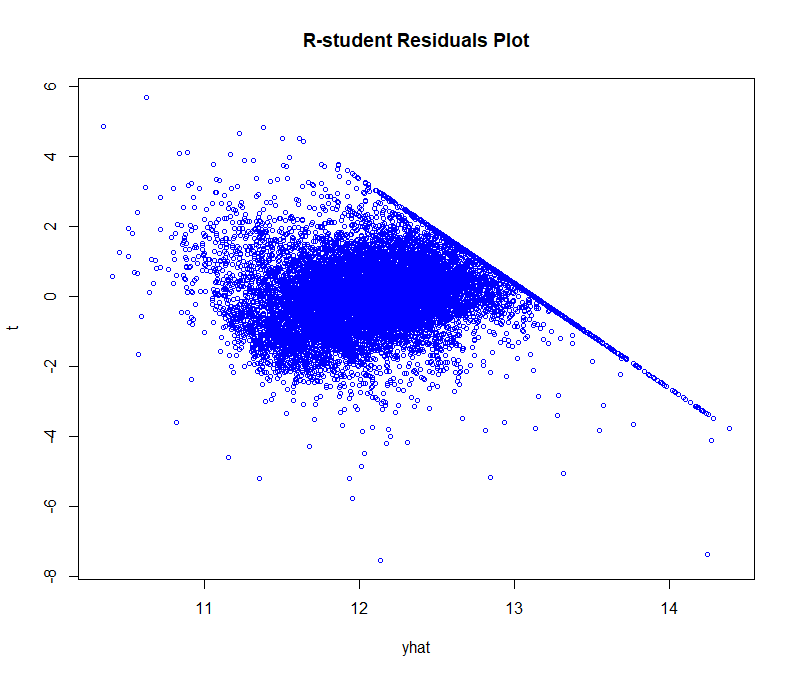
\includegraphics[width=7cm,height=6cm]{Rplot04.png}
		\caption{R-student Residuals Plot}
	\end{minipage}
	\begin{minipage}[t]{0.48\textwidth}
		\centering
		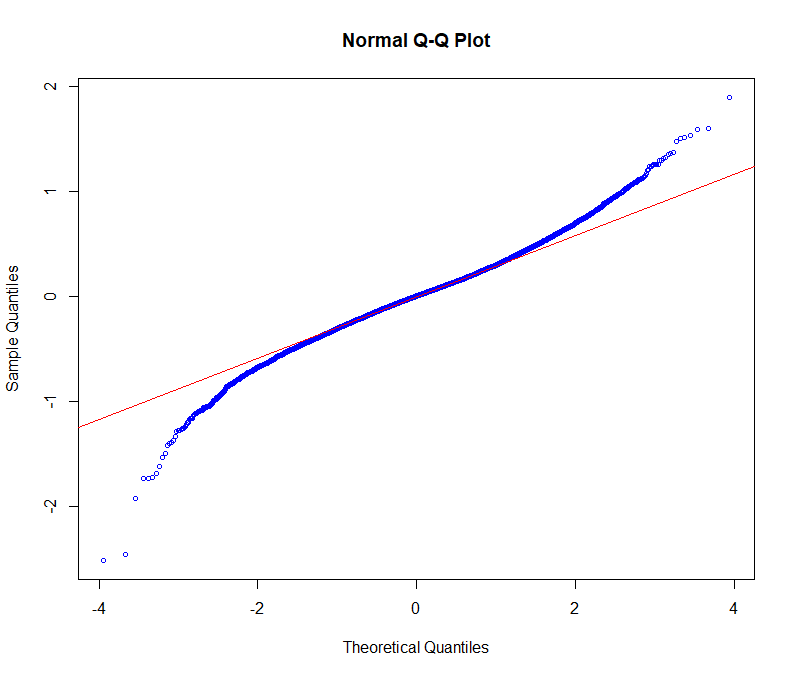
\includegraphics[width=7cm,height=6cm]{Rplot05.png}
		\caption{Normal QQ Plot}
	\end{minipage}                      
\end{figure}

\section{Polynomial Regression}
\qquad Then, we try to fit the polynomial regression model to training data set. Here we fix $K=2$ in the polynomial regression model. The regression model is 

\begin{equation}
y = \beta_{0}+\sum_{i=1}^{8}\beta_{i}x_{i}+\sum_{i=1}^{8}\beta_{ii}x_{i}^{2}+\sum_{j=1,k=1,j<k}^{8}\beta_{jk}x_{j}x_{k}+\varepsilon
\end{equation}
\indent After the LS fitting, we can get the value of all the parameters.
Then we construct t-test to test the significance of each parameter. Since some p-value are not close to 0, we eliminate those parameters in the model. We list them in the following table.
\begin{table}[h]
	\centering
	\begin{tabular}{ccccccccccc}
		\hline
		$\beta_{5}$ & $\beta_{6}$ & $\beta_{8}$ & $\beta_{16}$ & $\beta_{33}$ & $\beta_{35}$ & $\beta_{38}$ & $\beta_{47}$ & $\beta_{56}$ & $\beta_{67}$ & $\beta_{68}$ \\
		\hline
	\end{tabular}
	\caption{Eliminated Parameters in Polynomial Regression}
\end{table}

\indent In this model, $R^{2}=0.7235$, $R^{2}_{adj}=0.7227$ and $MSE=0.1467$. Now we conclude the merits and demerits of using the polynomial regression model.

\begin{itemize}
	\item Merits: consider the factors that combine effect of two or more variables, bring more functions which can be fit under it, make the prediction more precise.
	\item Demerits: may cause the problem of overfitting when the order is large; raise the probability of multicollinearity problem; model are quite sensitive to the outliers, which causes that few outliers in data can seriously affect results.
\end{itemize}

Then we try to fit the ridge regression model, that is, adding an $L_{2}$ regularization term to the cost function.

\begin{equation}
S(\beta)= \lVert X\beta-\bm{y}\rVert^{2}+\lambda\lVert\beta\rVert^{2}
\end{equation}

The best choice of parameter $\lambda$ is the one that makes the value of $MSE$ to be the smallest. We can compare them through GCV. Here we get the graph of the relation between GCV and $\lambda$. The graph is in Appendix.\\
\indent We can know that $MSE$ increases when $\lambda$ becomes larger. Thus adding an $L_{2}$ regularization term to the cost function dose not help decrease $MSE$. The probable reason is that the value of $\beta$ is not large in the original LS estimate, adding an $L_{2}$ term affect the precision of $\beta$ estimate.

\section{Nonlinear Regression} 
\qquad Then, we try to fit the polynomial regression model, namely the neural network (NN) model, to training data set.\\
\indent The neural network contains input layer, output layer, and hidden layers. Each layer contains some neurons. 

\subsection{Introduction of Neural Network}
\qquad Suppose the neural network contains $n$ layers, and thus the input layer is the $1^{st}$ layer, the output layer is the $n^{th}$ layer, the rest are hidden layers. The value of each neuron of the $i^{th}$ layer is computed by all the neurons of $(i-1)^{th}$ layer.\\
\indent Here are the equation for computation of each layer.

\begin{equation}
f_{j}^{(i+1)}=f\left(\sum_{k=1}^{m}\omega_{k}f_{k}^{(i)}+\theta_{j}\right)
\end{equation}
Note that in equation (4), $f_{j}^{(i+1)}$ is the value of the $j^{th}$ neuron from the $(i+1)^{th}$ layer, $m$ is the number of neurons from the $i^{th}$ layer, $\omega_{k}$ is the weight of $f_{k}^{(i)}$, and $\theta_{j}$ is the bias. Besides, $f$ is known as the activation function.\\
\indent When consider all the layers, the equation can be rewrite.

\begin{equation}
f(X;\theta)=f^{(n-1)}\left(\cdots f^{(3)}\left(f^{(2)}\left(f^{(1)}\left(X;W_{1}\right);W_{2}\right);W_{3}\right);W_{(n-1)}\right)
\end{equation}
Note that in equation (5), $f^{(i)}$ is different from equation (4), for the reason that both input and output are vectors. Here $X=(x_{1},x_{2},\dots,x_{n})$, which is the combination of all input variables. Here $W_{i}=(w_{i1},w{_{i2}},\dots,w_{in})$, where $n$ is the number of neurons from the $i^{th}$ layer. Besides, $\theta$ is the parameter in this model.

\subsubsection{Reason for Nonlinear Model}
\qquad Since the neural network contains several layers, even though the relation between adjacent layers is linear, after the combination of more than one hidden layers, the relation between input and output variables are nonlinear. Thus, the neural network is a kind of nonlinear model.
\subsubsection{Procedure of Training Data}
\qquad Then we illustrate the mechanism of the neural network. Giving the initial value of the parameter, model can give out the prediction of output, then through modifying the value of parameter, model can get the prediction of output more precisely, thus get the final training result. 

\subsection{Application of Neural Network}
\qquad Since it is better to normalize the data before applying model, we use min-max normalization here. By setting the layer neurons number as 8, 5, 3, 1, we can get the training result.
\begin{figure}[h]
	\centering
	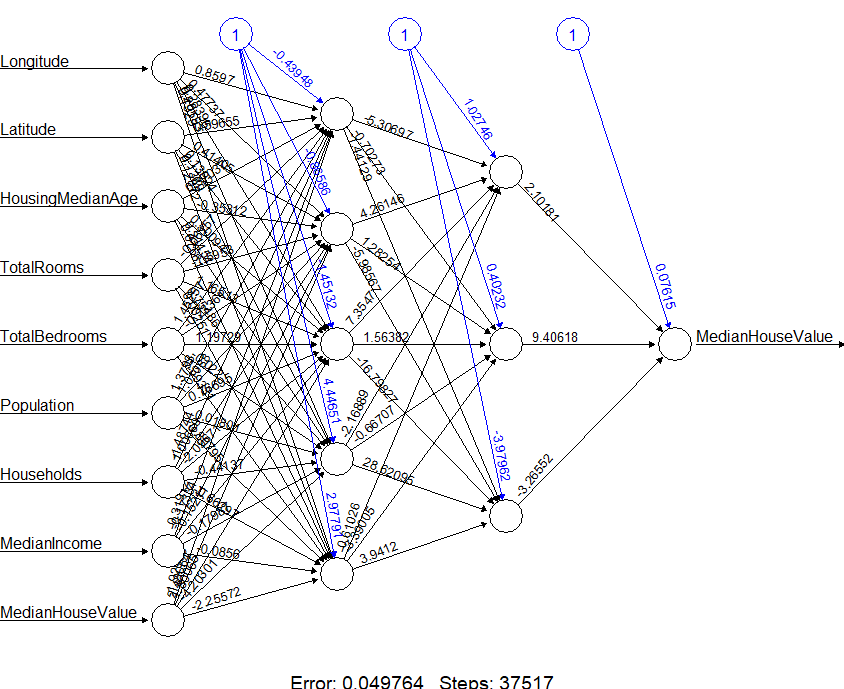
\includegraphics[width=10cm,height=7.5cm]{Rplot07.png}
	\caption{The Result of Neural Network Training}
\end{figure}

Note that the median house value is transformed to $ln$(median house value) in the training procedure. \\
\indent In this model, $R^{2}=0.99997$, where $R^{2}_{adj}$ is close to $R^{2}$, and $MSE=9.9235\times10^{-6}$. Both $R^{2}_{adj}$ and $MSE$ are much smaller than those of linear models. Now we conclude the merits and demerits of using the polynomial regression model. 

\begin{itemize}
	\item Merits: optimize the conventional model, enable the model become robust, make the prediction much more precise.
	\item Demerits: much more data have to be trained in order to construct the model; the complexity of algorithm increases; costs more time to get the final model; depends on computer to solve out the model.
\end{itemize}

\section{Alternating Conditional Expectation}
\qquad Now we try to use alternating conditional expectation (ACE) algorithm, which applies optimal transformation on both output and input variables of the original data set.\\
\indent In the ACE model, $R^{2}=0.7099$, where $R^{2}_{adj}$ is close to $R^{2}$, and $MSE=0.1493$. We can find that the $R^{2}_{adj}$ and $MSE$ are close to multiple and polynomial regression model, but differ quite a lot with NN model.\\
\indent Then we try to compare the residual plots of ACE model with those of the ordinary LS model which is constructed without performing data transformation.

\begin{figure}[h]
	\centering
	\begin{minipage}[h]{0.48\textwidth}
		\centering
		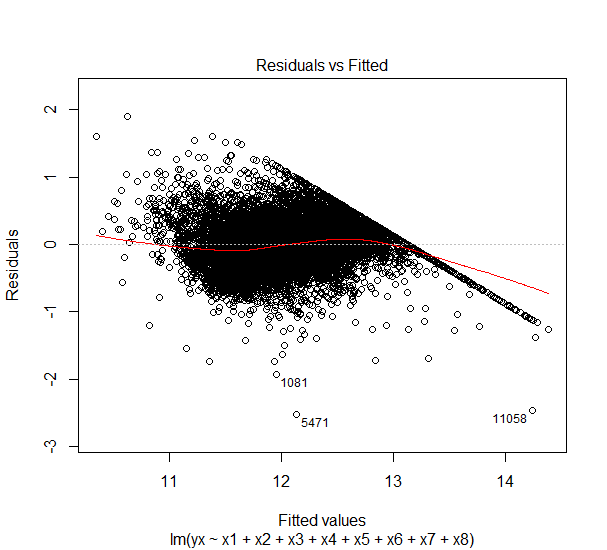
\includegraphics[width=6.5cm,height=6.5cm]{Rplot10.png}
		\caption{Residual Plot of Multiple Regression}
	\end{minipage}
	\begin{minipage}[h]{0.48\textwidth}
		\centering
		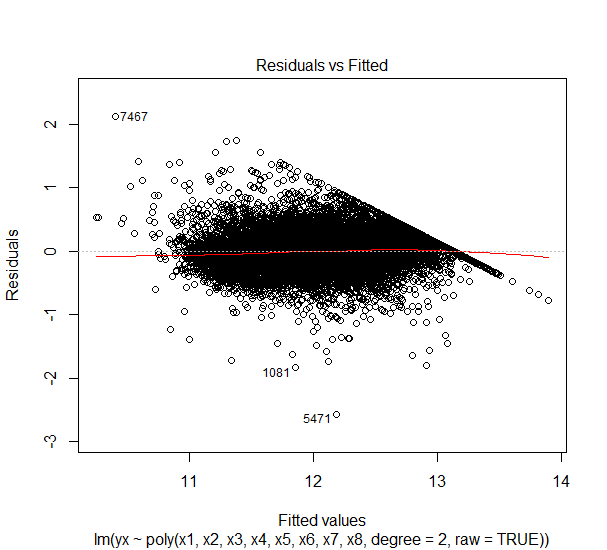
\includegraphics[width=6.5cm,height=6.5cm]{Rplot11.png}
		\caption{Residual Plot of Polynomial Regression}
	\end{minipage}                
\end{figure}
\begin{figure}[h]
	\centering
	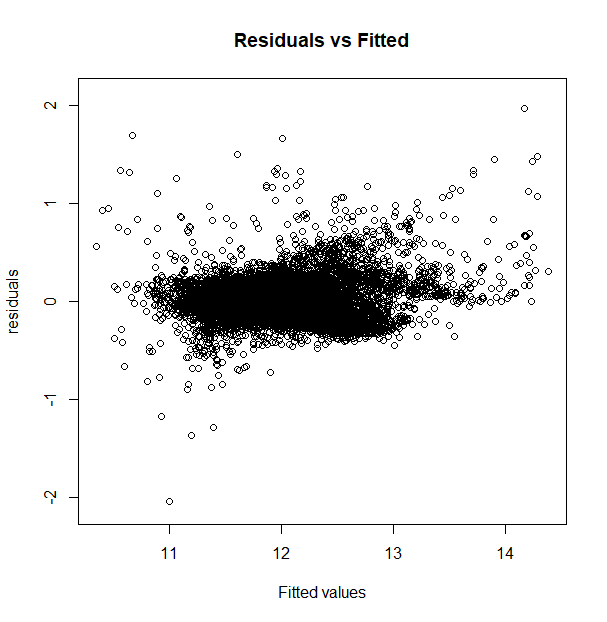
\includegraphics[width=7.5cm,height=7.5cm]{Rplot12.png}
	\caption{Residual Plot of ACE Model}
\end{figure}
\indent In figure 4, 5 and 6, we can see that the residuals are concentrated around the line $y=0$, and the bound line becomes vague. In this question, we can not conclude that the ACE model is superior to multiple linear regression model, for the reason that they are close in terms of performances. But we can not deny that ACE model may be superior in solving other questions. The judgment depends on case being studied. \\ 
\indent Now we discuss the merits and demerits of using ACE model.

\begin{itemize}
	\item Merits: optimize the conventional model , make the training and prediction precise.
	\item Demerits: the algorithm complexity increases; costs much more time to construct model; sensitive to outliers; depends on computer to solve out the model.
\end{itemize}


\section{Outliers}
\qquad In this section, we focus on the outliers in data set. Here we apply Cook's measure to training data to identify the outliers, or more precisely, influential points.\\
\indent We choose the models mentioned before to help identify outliers, including multiple linear regression model and polynomial regression model. Note that we preserve all the parameters in polynomial regression here.\\
\indent The following graphs show the leverage of each residual points. The left side is from multiple linear regression, and the right side is from polynomial regression.

\begin{figure}[h]
	\centering
	\begin{minipage}[h]{0.48\textwidth}
		\centering
		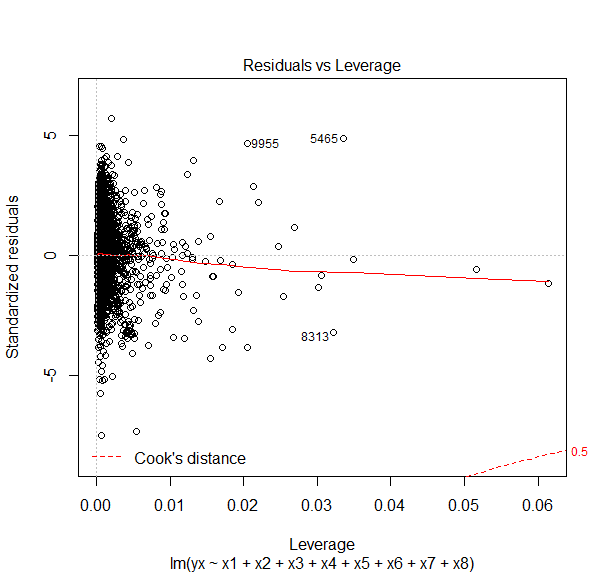
\includegraphics[width=7.5cm,height=7.5cm]{Rplot08.png}
		\caption{QQ Plots of Variables}
	\end{minipage}
	\begin{minipage}[h]{0.48\textwidth}
		\centering
		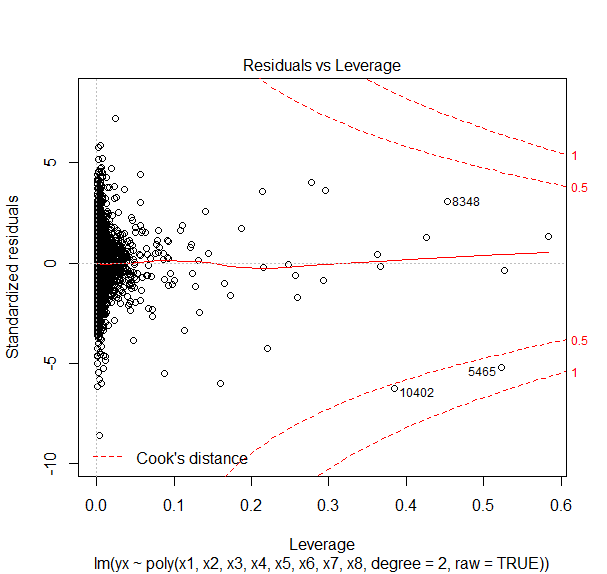
\includegraphics[width=7.5cm,height=7.5cm]{Rplot09.png}
		\caption{Histograms of Variables}
	\end{minipage}                      
\end{figure}

In Figure 4, we can see that all the residual points are within Cook's distance, which roughly implies that no influential points in this model. In Figure 5, we can see that 2 residual points are outside Cook's distance, which implies these data points are influential in the regression procedure of this model. Also, most of the residual points are within the range (-2,2). So far, we can conclude that only a small fraction of data are outliers.\\
\indent Now we discuss the way to achieve robustness against outliers. We can just follow the steps to build robust regression model. (1) delete the data points which are within Cook's distance; (2) consider of the data points which are outside Cook's distance, and think about whether they are subject to "men-made" errors, if so, then just delete, otherwise, keep them in the data set; (3) rebuild the regression model. However, we can also use other way to achieve robustness, like applying NN model and ACE model which are more complex.

\section{Comparison}
\qquad In this section, we try to make comparison of different regression models in terms of some kinds of indicators. In order to see the comparison visually, here we make a table for the comparison results from this question. \\

\begin{table}[h]
	%\centering
	\begin{tabular}{ccccc}
		\hline
		& Multiple Model & Polynomial Model & NN Model & ACE Model \\
		\hline
		Training Performance & $\checkmark$ & $\checkmark\checkmark$ & $\checkmark\checkmark\checkmark\checkmark\checkmark$ &  $\checkmark\checkmark$ \\
		Prediction Performance & $\checkmark\checkmark$ & $\checkmark$ & $\checkmark\checkmark\checkmark\checkmark\checkmark$ & $\checkmark\checkmark$ \\
		Overfitting & $\smallsetminus$ & $\checkmark$ & $\checkmark$ & $\checkmark$ \\
		Time Complexity & $\checkmark$ & $\checkmark\checkmark$ & $\checkmark\checkmark\checkmark\checkmark$ & $\checkmark\checkmark\checkmark\checkmark\checkmark$\\
		Outliers Sensitivity & $\checkmark\checkmark\checkmark$ & $\checkmark\checkmark\checkmark$ & $\checkmark$ & $\checkmark\checkmark\checkmark$ \\
		\hline
	\end{tabular}
	\caption{Comparison of Regression Models}
\end{table}
Note that in Table 5, more ticks means the certain model achieve more on the indicator which is labeled on the left, like better training performance, better prediction performance, consuming more time, and more sensitive to outliers. Besides, we can see that, except for multiple linear regression model, it is possible for all the other models to have the problem of overfitting.

\section{Summary}
\qquad In this section, we make a summary of the main findings obtained from solving the above regression models. 

\begin{itemize}
	\item In general, nonlinear models have better performances than linear models, that is, nonlinear models are more useful, which can be reflected in training and prediction performance.
	\item Overfitting problem exits in most regression models, remember to be avoid of making the model too complex, which can help keep from overfitting.
	\item Outliers problem have an effect on all the models, however, a compromise between deleting outliers and retaining outliers can leads to robust regression.
    \item Data normalization enable the procedure of dealing with data to be more easy, it is better to normalize the data set before applying regression.
    \item The training performance is not certainly related with prediction performance, due to the uncertainty of data, model with good training performance may have bad prediction performance and vice versa.
    \item In the above models, there exists a balance between model performance and model time complexity, that is, achieving better results needs more time to training the data.
\end{itemize}

\newpage 
\appendix
\section{Appendix}
\begin{figure}[h]
	\centering
	\begin{minipage}[h]{0.48\textwidth}
		\centering
		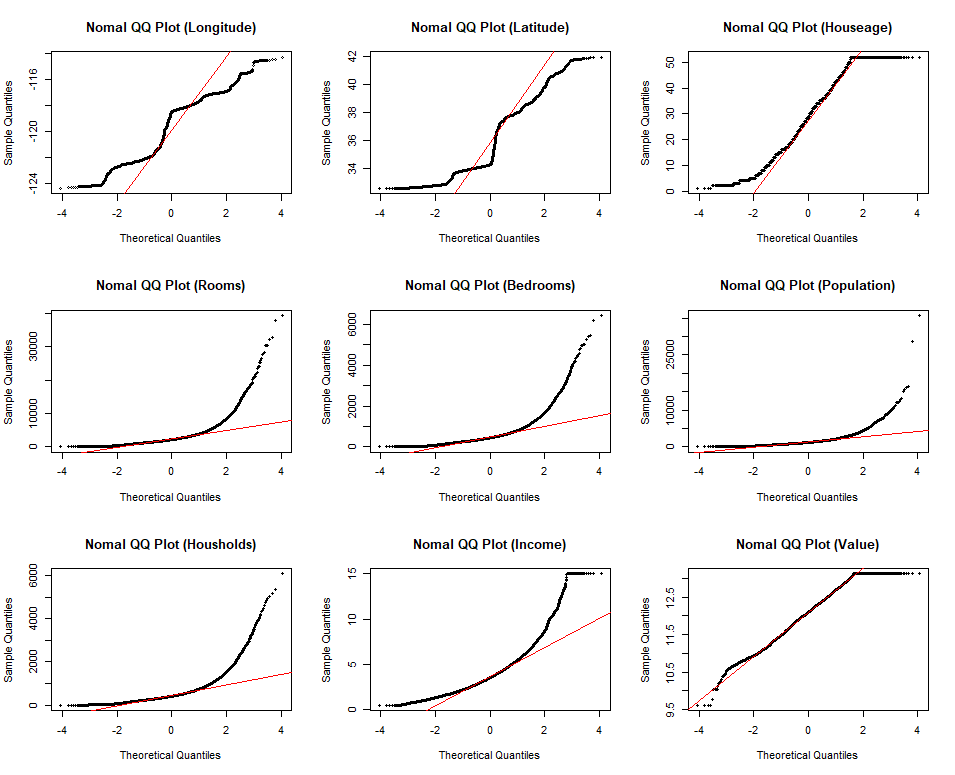
\includegraphics[width=7.5cm,height=7.5cm]{Rplot01.png}
		\caption{QQ Plots of Variables}
	\end{minipage}
	\begin{minipage}[h]{0.48\textwidth}
		\centering
		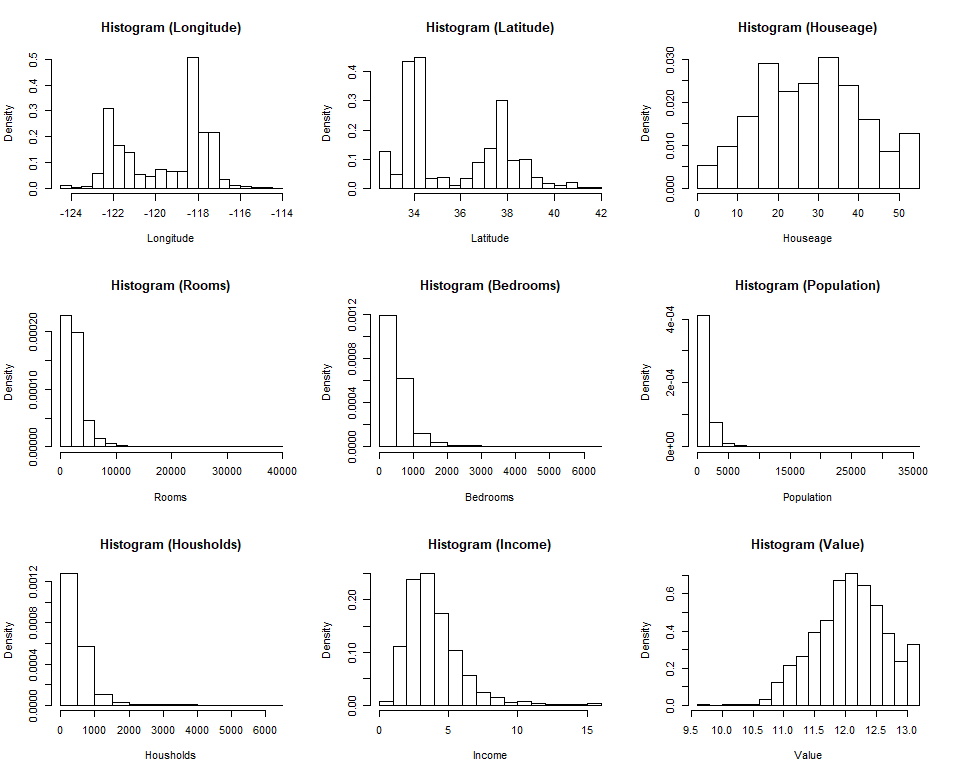
\includegraphics[width=7.5cm,height=7.5cm]{Rplot02.png}
		\caption{Histograms of Variables}
	\end{minipage}                      
\end{figure}

\begin{figure}[h]
	\centering
	\begin{minipage}[h]{0.48\textwidth}
		\centering
		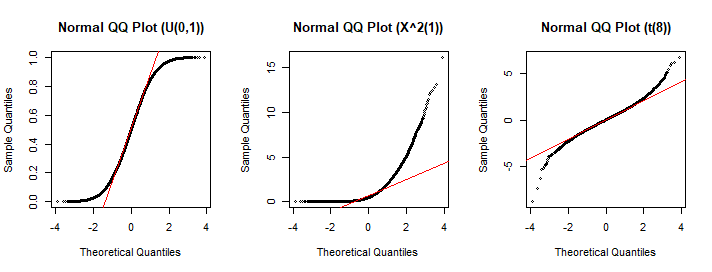
\includegraphics[width=7.5cm,height=3.5cm]{Rplot03.png}
		\caption{QQ Plots of Common Distributions}
	\end{minipage}
	\begin{minipage}[h]{0.48\textwidth}
		\centering
		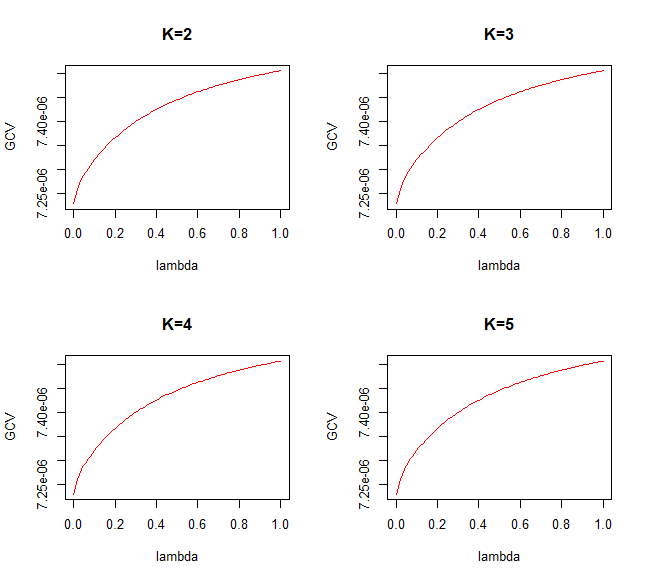
\includegraphics[width=7.5cm,height=6.5cm]{Rplot06.png}
		\caption{Relation of GCV and $\lambda$}
	\end{minipage}                      
\end{figure}

\end{document}

